\section{Introduction}\label{sec:introduction}
This project is part of a solar-powered e-bike charging station that will be built on the campus of Delft University of Technology. This station consists of power electronics to manage power between the solar panels, the station batteries, the grid and all the connected vehicles. The station is able to charge e-bikes both wired and wirelessly, as well as e-scooters. The station also has a weather station to monitor the outside climate. Furthermore, the system has a number of temperature sensors to monitor the temperature levels of the solar panels. A concept of the station can be found in \Cref{fig:station_concept}.

\begin{figure}[!ht]
  \centering
    \includegraphics[width=0.6\textwidth]{images/charging_station.png}
      \caption{Concept of the solar powered e-bike charging station \cite{feasibility_study}}\label{fig:station_concept}
\end{figure}

The SUNRISE project (Smart Unified Networking Rig for an Integrated Solar E-bike charger) was proposed as a final BSc project. The result of this project should manage the data generated by the power electronics, weather station and temperature probes through a local mini computer and log the information on a TU Delft server. This mini computer should also control a local display that shows live information about the system. SUNRISE should also be able to handle requests of registered users that want to charge their vehicle at the station. The input is processed through a webpage hosted by the university, which should trigger the station to turn on one of the chargers. The webpage will then comunicate to the user what charger to use, after which the user will be able to monitor the state of their battery through the webpage. Finally, the SUNRISE project should have an administrator dashboard to show the status and data of the system, and a media webpage that will display some basic information to the media. An overview of the entire system can be found in \Cref{fig:project_overview}.

\begin{figure}[!ht]
  \centering
    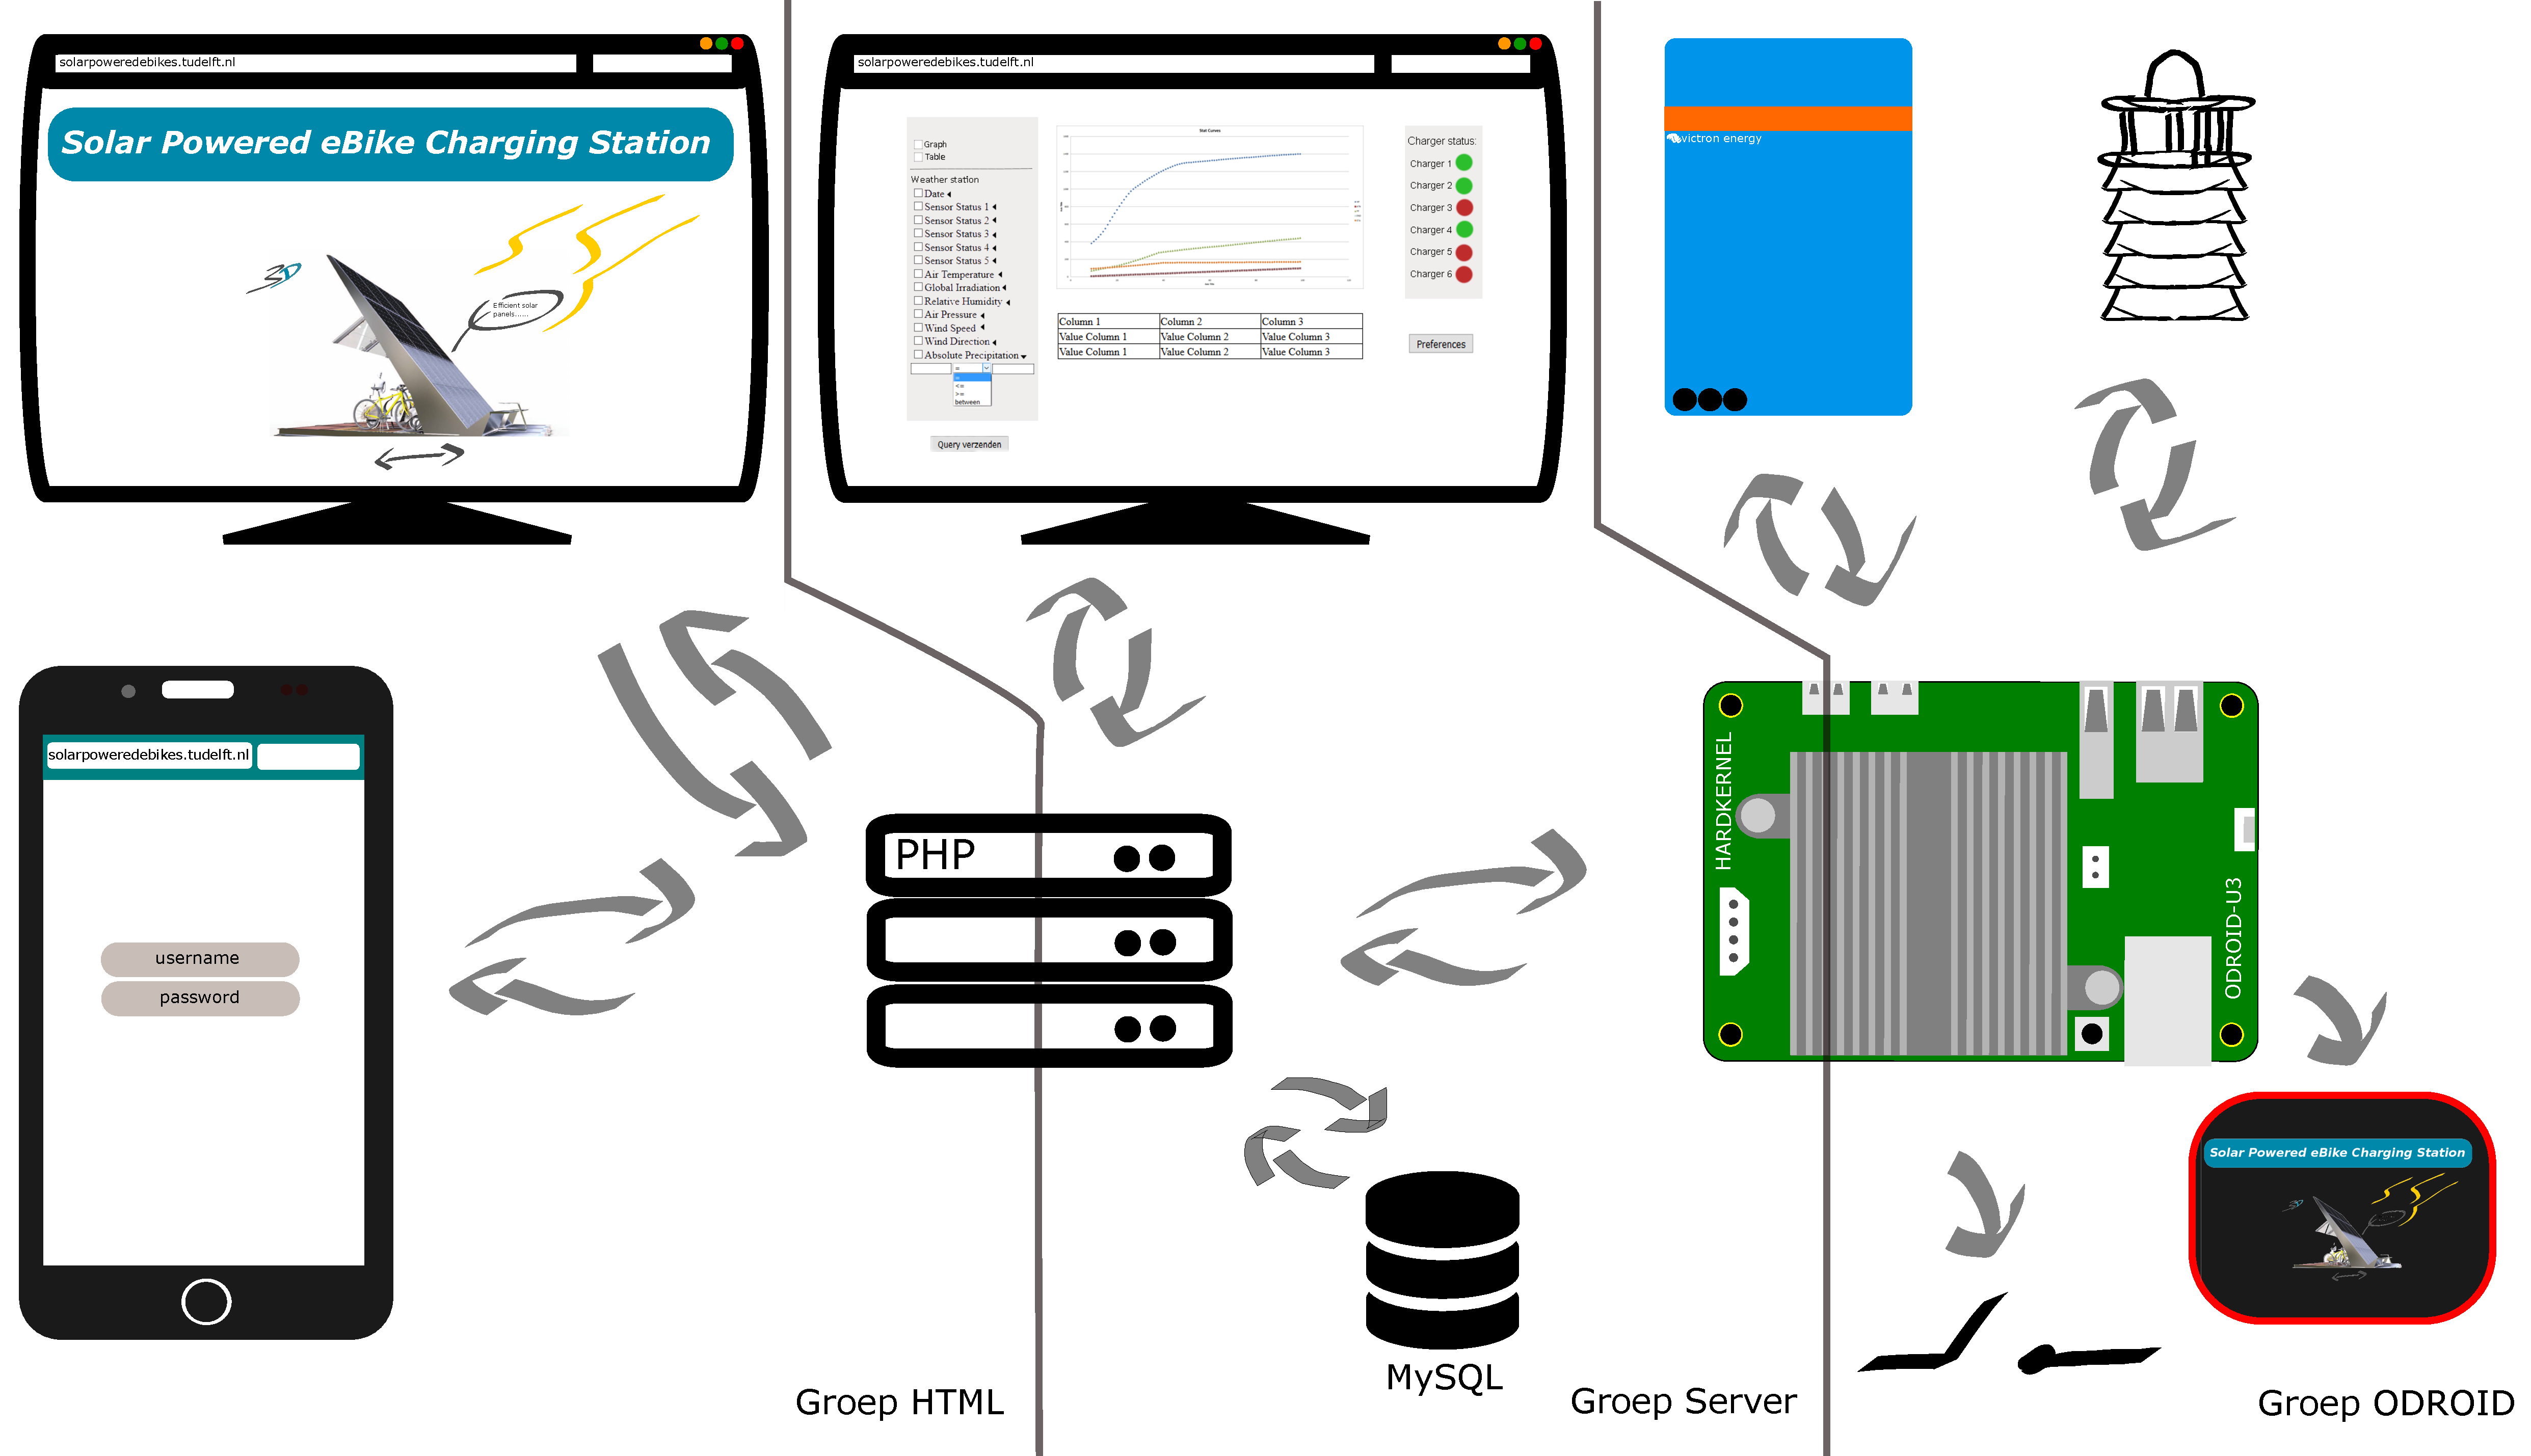
\includegraphics[width=1.0\textwidth]{images/project_overview.pdf}
      \caption{An overall view of the entire SUNRISE system}\label{fig:project_overview}
\end{figure}